
\subsection{Herramienta Utilizadas} 
    

\subsubsection*{Kali Linux}
Kali Linux es una distribución de Linux (basada en Debian) centrada en la seguridad. 
Es una versión renombrada de la famosa distribución de Linux conocida como Backtrack, 
que venía con un enorme repositorio de herramientas de piratería de código abierto, 
para pruebas de penetración de aplicaciones \emph{web}, inalámbricas y de red. 

\begin{center}
    \begin{figure}   
       \begin{center}
          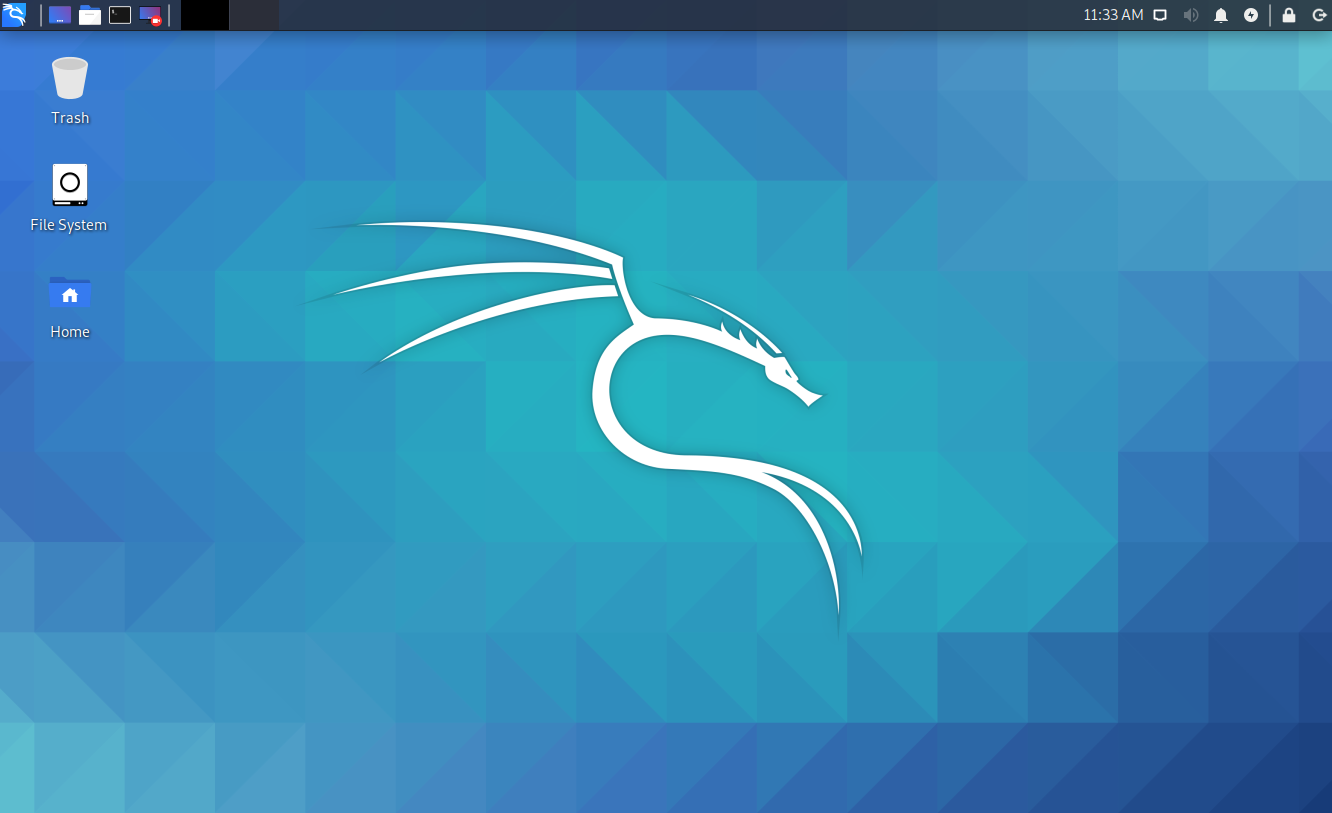
\includegraphics[width=11cm,height=7cm]{ataque-1.png}
       \end{center}
       \caption{Escritorio de Kali Linux}
    \end{figure}
 \end{center}
 

Kali Linux contiene muchas herramientas preinstaladas con 
todas las dependencias y ya está lista para usar. Esto nos permite tener que prestar 
más atención a las pruebas y no a la instalación de la herramienta. Las actualizaciones 
para las herramientas instaladas en Kali Linux se publican con mayor frecuencia, 
lo que le ayuda a mantener las a las mismas actualizadas.

Esta distribución contiene las herramientas necesarias para realizar nuestro
ataque.

\subsubsection*{Wireshark}
Wireshark es uno de los analizadores de protocolos de red más populares, es de 
código abierto y gratuito. Wireshark está preinstalado en Kali y es ideal para la 
resolución de problemas de red, análisis y, para este caso de estudio, una herramienta 
perfecta para monitorear el tráfico de posibles objetivos. Wireshark usa un kit de 
herramientas para implementar su interfaz de usuario y para capturar paquetes. 
Funciona de manera muy similar a un comando \emph{tcpdump}; sin embargo, nos brinda
una interfaz gráfica, posee opciones integradas de clasificación y filtrado.

\begin{center}
    \begin{figure}   
       \begin{center}
          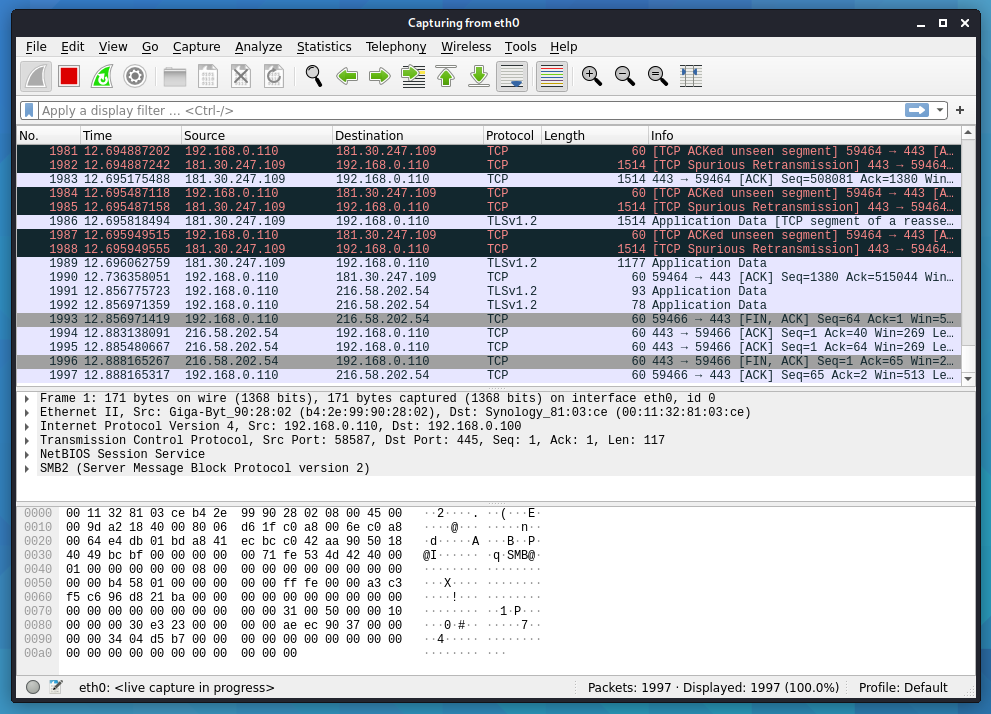
\includegraphics[width=10cm,height=7cm]{wireshark.png}
       \end{center}
       \caption{Interface del Wireshark}
    \end{figure}
 \end{center}
 
\subsubsection*{Ettercap}

\begin{center}
   \begin{figure}   
      \begin{center}
         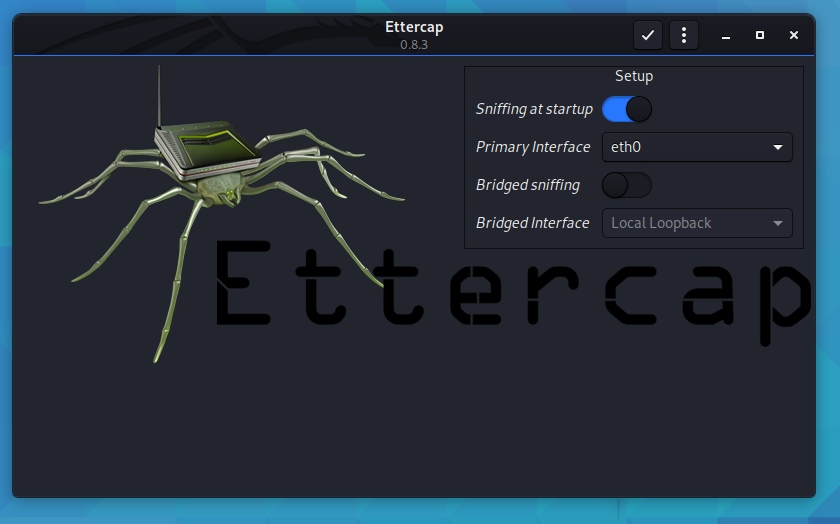
\includegraphics[width=10 cm,height=7cm]{ataque-2.png}
      \end{center}
      \caption{Ettercap}
   \end{figure}
\end{center}

Ettercap es un paquete completo gratuito y de código abierto para ataques basados 
en intermediarios. Ettercap se puede utilizar para análisis de protocolos de redes 
informáticas y auditorías de seguridad, con funciones de rastreo de conexiones en 
tiempo real y filtrado de contenido. Ettercap funciona configurando la interfaz de red 
del atacante en modo promiscuo y \emph{ARP} para envenenar las máquinas víctimas.



(HAY MAS, CON GRAFICOS EN)
Joseph Muniz, Aamir Lakhani - Web Penetration Testing with Kali Linux-Packt Publishing (2013)
Aca yo segui un tutorial, buscarlo
\subsection{Realización del ataque}
La idea principal de esta sección es demostrar que, encontrandose en una red interna
y con con herramientas ya desarrolladas y libres es posible realizar un ataque 
sin necesidad de conocer a fondo la implementacion de la misma ni de tener mayores
privilegios

Recordar que esto fue realizado en una red interna donde son todos equipos de nuestra propiedad


IMAGEN de le red

Tiene que estar:
-Router

-Origen de la pagina

-Consumidor de la pagina

-El atacante

\subsection{Preparando Ettercap para el ataque ARP Poisoning}

Lo primero que debemos hacer, en la lista de aplicaciones, es buscar el apartado 
«9. Sniffing y Spoofing«, ya que es allí donde encontraremos las herramientas necesarias
 para llevar a cabo este ataque.

IMAGEN Kali Linux Spoofing

A continuación, abriremos «Ettercap» y veremos una ventana similar a la siguiente.

IMAGEN  Kali Linux Ettercap

El siguiente paso es seleccionar la tarjeta de red con la que vamos a trabajar. Para ello, en el menú superior de Ettercap seleccionaremos «Sniff > Unified Sniffing» y, cuando nos lo pregunte, seleccionaremos nuestra tarjeta de red (por ejemplo, en nuestro caso, eth0).

IMAGEN Kali Linux - Ettercap - Tarjeta de red

El siguiente paso es buscar todos los hosts conectados a nuestra red local. Para ello, seleccionaremos «Hosts» del menú de la parte superior y seleccionaremos la primera opción, «Hosts List«.

IMAGEN Kali Linux - Ettercap - Lista de hosts

Aquí deberían salirnos todos los hosts o dispositivos conectados a nuestra red. Sin embargo, en caso de que no salgan todos, podemos realizar una exploración completa de la red simplemente abriendo el menú «Hosts» y seleccionando la opción «Scan for hosts«. Tras unos segundos, la lista de antes se debería actualizar mostrando todos los dispositivos, con sus respectivas IPs y MACs, conectados a nuestra red.

IMAGEN Kali Linux - Ettercap - Lista de hosts 2

\subsection{Nuestro Ettercap ya está listo. Ya podemos empezar con el ataque ARP Poisoning}

En caso de querer realizar un ataque dirigido contra un solo host, por ejemplo, suplantar la identidad de la puerta de enlace para monitorizar las conexiones del iPad que nos aparece en la lista de dispositivos, antes de empezar con el ataque debemos establecer los dos objetivos.

Para ello, debajo de la lista de hosts podemos ver tres botones, aunque nosotros prestaremos atención a los dos últimos:

    Target 1 – Seleccionamos la IP del dispositivo a monitorizar, en este caso, el iPad, y pulsamos sobre dicho botón.
    Target 2 – Pulsamos la IP que queremos suplantar, en este caso, la de la puerta de enlace.

IMAGEN Objetivos Ettercap

Todo listo. Ahora solo debemos elegir el menú «MITM» de la parte superior y, en él, escoger la opción «ARP Poisoning«.

IMAGEN Kali Linux - Ettercap - Ataques MITM

Nos aparecerá una pequeña ventana de configuración, en la cual debemos asegurarnos de marcar «Sniff Remote Connections«.

IMAGEN Comenzar MITM ARP Poisoning

Pulsamos sobre «Ok» y el ataque dará lugar. Ahora ya podemos tener el control sobre el host que hayamos establecido como «Target 1«. Lo siguiente que debemos hacer es, por ejemplo, ejecutar Wireshark para capturar todos los paquetes de red y analizarlos en busca de información interesante o recurrir a los diferentes plugins que nos ofrece Ettercap, como, por ejemplo, el navegador web remoto, donde nos cargará todas las webs que visite el objetivo.

Plugins Ettercap
